%%%%%%%%%%%%%%%%%%%%%%%%%%%%%%%%%%%%%%%%
%%%%%  xPhO LaTeX Beamer Template  %%%%%
%%%%%  Date: 17/03/2025            %%%%%
%%%%%  Authors:                    %%%%%
%%%%%       Nguyen Thanh Long      %%%%%
%%%%%       Nguyen Le Mai Huong    %%%%%
%%%%%       Nguyen Minh Phuong     %%%%%
%%%%%%%%%%%%%%%%%%%%%%%%%%%%%%%%%%%%%%%%

\documentclass[aspectratio=169, t]{beamer} % Ratio 16:9
\usepackage[T5]{fontenc}
\usepackage{lmodern}
\usepackage{graphicx} 
\usepackage{array}
\usepackage{longtable} % for long table
\usepackage{chngcntr}
\counterwithin{figure}{section}
\usepackage{tcolorbox}
\renewcommand{\familydefault}{\sfdefault} % Font

\usepackage{caption}
\usepackage{siunitx}

\usepackage{tikz}
\usetikzlibrary{patterns}
\usepackage{subcaption}
\let\vec\relax
\newcommand{\vec}[1]{\textbf{#1}}

\usepackage{multicol}

\usepackage{mdframed}

% \definecolor{BlueDefault}{rgb}{0.2,0.2,0.7}
\definecolor{BlueDefault}{RGB}{14,47,95}


% Hide navigation 
\setbeamertemplate{navigation symbols}{}

% Setup background
\newcommand{\normalbackground}{%
    \usebackgroundtemplate{
\includegraphics[width=\paperwidth,height=\paperheight]{Background/Normal_slide_xPhO.pdf}}%
}

\newcommand{\titlebackground}{%
    \usebackgroundtemplate{
\includegraphics[width=\paperwidth,height=\paperheight]{Background/Title_slide_xPhO.pdf}}%
}

% Change the title color to white
\setbeamercolor{frametitle}{fg=white} 

% push the title up by \raisebox
\setbeamertemplate{frametitle}{%
    \vspace{0.3em}
    \hspace{-1em} \insertframetitle
    \vspace{2mm}
}

% Number of slide
\setbeamertemplate{footline}{%
    \hfill
    \insertframenumber/\inserttotalframenumber
    \hspace{7.5mm}
    \vspace{3.5mm}
}

%% Make Table of Contents %%
\AtBeginSection[]{
    \begin{frame}
        \frametitle{Mục lục}
            \tableofcontents[currentsubsection]
    \end{frame}
}

%% Section numbering %%
\setbeamertemplate{section in toc}[sections numbered]
\setbeamertemplate{subsection in toc}[subsections numbered]


\renewcommand{\figurename}{Hình}
\renewcommand{\tablename}{Bảng}

%%%%%%%%%% Pictures drawing %%%%%%%%%%%%%

\usepackage{pgfplots} %%%%%% Regression %%%%
\pgfplotsset{compat = newest}
\usepackage{pgfplotstable}
\usepackage{tikz}
\usepackage{tikz-3dplot} %%%%%% Draw %%%%%%
\usepackage{tikz,tkz-euclide}
\usetikzlibrary{arrows,calc,patterns}
\usetikzlibrary{quotes,angles}
\usetikzlibrary{shapes.geometric}
\usepackage{circuitikz} %%%%% Circuit %%%%
\usetikzlibrary{decorations.pathmorphing,patterns}


%%%%% Bibliography %%%%%
\usepackage[backend=biber,style=ieee]{biblatex}
\addbibresource{citation.bib}

\usepackage{url}
\usepackage{hyperref}
\hypersetup{
	colorlinks=true,
	linkcolor=BlueDefault,
	filecolor=BlueDefault,
    citecolor=BlueDefault,
	urlcolor=BlueDefault,
	pdftitle={Overleaf Example},
	pdfpagemode=FullScreen,
}

%%%%%%%%%% Color setup %%%%%%%%%%%%%

\RequirePackage{xcolor}
\definecolor{wsdred}{HTML}{8E1728}
\definecolor{wsdgrey}{HTML}{75787B}
\renewcommand{\normalcolor}{\color{wsdred}}
\colorlet{ColorOr}{white}

\begin{document}

\titlebackground

\begin{frame}[noframenumbering]
    \thispagestyle{empty}
    \bfseries
    \begin{flushleft}
        \vfill
        \vspace{5mm}
        \textcolor{BlueDefault}{\huge \bfseries Vector và  \\Nhập môn Đại số tuyến tính} \\
        \vspace{8mm}
        \textcolor{black}{\large \bfseries Người trình bày: Carina }
        \vfill
    \end{flushleft}
\end{frame}

\normalbackground

\section{Vấn đề khởi động}
\begin{frame}
    \frametitle{Bài toán khởi động}
    \begin{columns}
        \begin{column}{0.5\textwidth}
            \vspace{-16pt}

            \begin{figure}
                \centering
                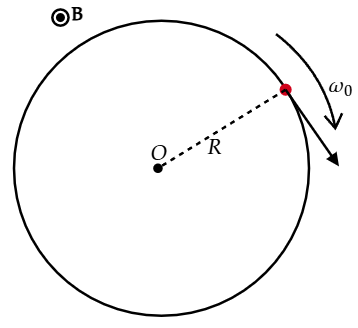
\includegraphics[width=3.5cm, height=3.5cm]{Content/Figure/initial_motion.png}   
                \caption{Chuyển động ban đầu}
            \end{figure}
            \begin{itemize}
                \item  \(\mathbf{B}=\frac{B_0}{r^n}\hat{z}\).
                \item \(\omega_0 =\frac{eB_0}{mR^n}\).
            \end{itemize}
           
        \end{column}
        \begin{column}{0.5\textwidth}
            \vspace{-2pt}

            \begin{figure}
                \centering
                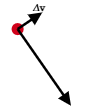
\includegraphics[width=2cm, height=3cm]{Content/Figure/initial_motion2.png}
                \caption{Nhiễu động nhỏ}
            \end{figure}
            \begin{itemize}
                \item \(\lvert\Delta\mathbf{v}\rvert \ll\omega_0 R\).
                \item \(r_{\text{max}}=R+\delta,\quad \delta\ll R\).
            \end{itemize}
        \end{column}
    \end{columns}
\end{frame}
\begin{frame}
    \frametitle{Lời giải}
    Từ định luật II Newton và định luật Lorentz: \[m\mathbf{a}=e\mathbf{v}\times\mathbf{B}.\]
    Kết quả thu được: 
    \begin{equation}\label{eq1}
    \mathbf{a}=\begin{bmatrix}
        \ddot{r}-r\dot{\phi}^2\\
        r\ddot{\phi}+2\dot{r}\dot{\phi}\\
        \ddot{z}
    \end{bmatrix}=\frac{eB_0}{m}\begin{bmatrix}
        r^{1-n}\dot\phi\\
        -r^{-n}\dot{r}\\
        0
    \end{bmatrix}.
    \end{equation}
\end{frame}
\begin{frame}
    \frametitle{Lời giải}
    Chú ý rằng, \[r\ddot{\phi}+2\dot{r}\dot{\phi}=\frac{1}{r}\frac{d}{dt}(r^2 \dot\phi).\]
    Kết hợp với phương trình~\eqref{eq1}, và thu được
    \[\frac{d}{dt}\left(r^2\dot\phi +\frac{1}{2-n}\frac{eB_0}{m}r^{2-n}\right)=0.\]
    Hay, \[r^2\dot\phi +\frac{1}{2-n}\frac{eB_0}{m}r^{2-n}=const.~~(!)\]
    Kết quả cuối cùng: \begin{equation}
        r=R+\delta\cos\left(\omega_0\sqrt{1-n} t+\frac{\pi}{2}\right).
    \end{equation}
\end{frame}


\section{Các định luật bảo toàn}
\subsection{Động lượng}
\begin{frame}
    \frametitle{Hệ chất điểm}
    Hệ chất điểm là tập hợp của \(N\) chất điểm \(M_i\) có khối lượng \(m_i\) và vận tốc \(\mathbf{v}_i\), \(i=1,2,\ldots,N\).

    Ta định nghĩa khối tâm \(G\) của hệ chất điểm là điểm sao cho
    \begin{equation}
    \Sigma_i m_i \mathbf{GM_i} = 0.
    \end{equation}
    Khi đó,
    \begin{equation}
    \mathbf{OG} = \frac{\Sigma_i m_i \mathbf{OM_i}}{m}.
    \end{equation}
    và
    \begin{equation}
        \mathbf p=\Sigma_i m_i \mathbf{v}_i = m\mathbf{v_G}.
    \end{equation}
    Trong đó \(m=\Sigma_i m_i\) và \(\mathbf p\) là khối lượng và động lượng toàn phần của hệ.
\end{frame}

\begin{frame}
    \frametitle{Định luật II Newton cho hệ chất điểm}
    Định luật II Newton cho hệ chất điểm:
    \begin{equation}
        \frac{d\mathbf p}{dt} = \Sigma_i \mathbf{F}_i + \Sigma_i \Sigma_{j\neq i} \mathbf{f}_{ij}.
    \end{equation}
    Trong đó \(\mathbf{F}_i\) là ngoại lực tác dụng lên \(M_i\), và \(\mathbf{f}_{ij}\) là lực do \(M_j\) tác dụng lên \(M_i\).

    Số hạng thứ hai trong vế phải bằng 0 do định luật III Newton:
    \begin{equation}
        \frac{d\mathbf p}{dt}=\Sigma_i \mathbf{F}_i=m\mathbf{a_G}.
    \end{equation}
    Nếu tổng hợp lực ngoài tác dụng lên hệ bằng không, thì động lượng toàn phần của hệ được bảo toàn:
        \begin{equation}
            \mathbf p = const.
        \end{equation}
\end{frame}

\begin{frame}
\frametitle{Bài toán tên lửa}
Xét một tên lửa có tổng khối lượng \(m\) đang bay trong vũ trụ với vận tốc \(v\). Nhiên liệu được phóng ra sau một cách từ từ với vận tốc \(u\) so với tên lửa. Tính độ tăng vận tốc của tên lửa sau khi nó xả được một khối lượng nhiên liệu \(\Delta m\).
\vspace{1cm}
\begin{figure}
    \centering
    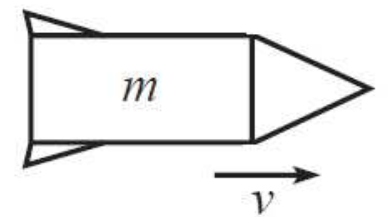
\includegraphics[width=0.3\textwidth]{Content/Figure/rocket.png}
\end{figure}
\end{frame}

\begin{frame}
\frametitle{Bài toán tên lửa}
\begin{columns}
\begin{column}{0.5\textwidth}
\begin{figure}
    \centering
    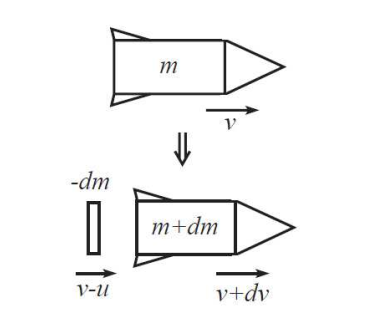
\includegraphics[width=0.6\textwidth]{Content/Figure/rocketsolving.png}
\end{figure}
Áp dụng định luật bảo toàn động lượng:
\begin{equation*}
    mv = (m+ dm)(v+dv) + (-dm)(v-u).
\end{equation*}
\end{column}
\begin{column}{0.5\textwidth}
    Ta suy ra được tích phân:
    \begin{equation}
        \int_{v}^{v+\Delta v} dv =- u \int_{m}^{m-\Delta m} \frac{dm}{m}.
    \end{equation}
    Từ đó ta thu được \(\Delta v\):
    \begin{equation}
        \Delta v = u \ln{\frac{m}{m-\Delta m}}.
    \end{equation}
\end{column}
\end{columns}
\end{frame}
\subsection{Năng lượng}
\begin{frame}
    \frametitle{Các bài toán quen thuộc}
    \begin{columns}
        \begin{column}{0.5\textwidth}
            \vspace{-14pt}

            \begin{figure}
                \centering
                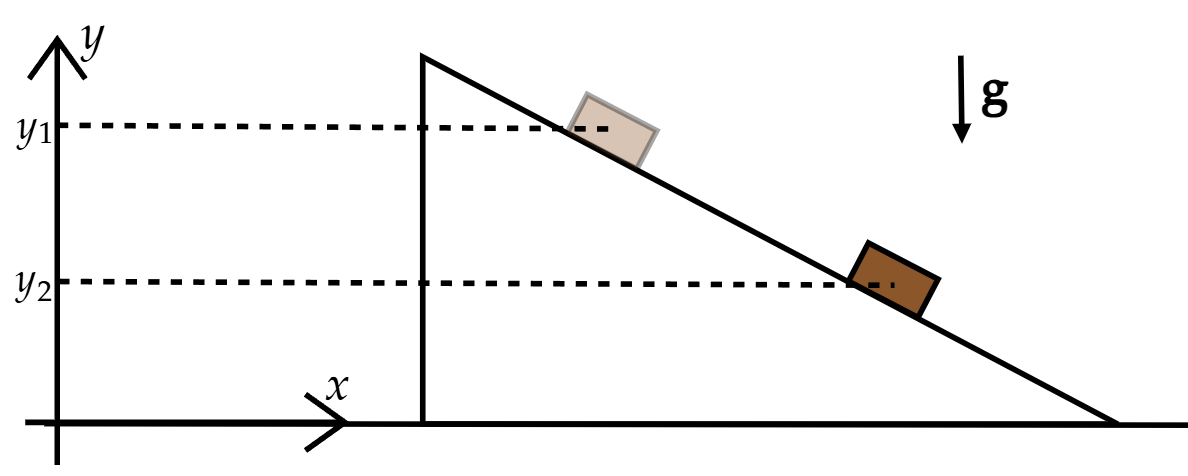
\includegraphics[width=7cm, height=3cm]{Content/Figure/gravity_energy.png}
            \end{figure}
            \[\frac{d}{dt}\left(\frac{mv^2}{2}-mgy\right)=0.\]
            \[\Delta\left(\frac{mv^2}{2}\right)-\int_{y_1}^{y_2}(-mg)dy=0.\]
        \end{column}
        \begin{column}{0.5\textwidth}
            \vspace{-14pt}

            \begin{figure}
                \centering
                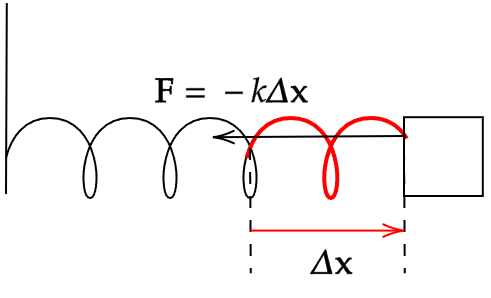
\includegraphics[width=5cm, height=3cm]{Content/Figure/springmass.png}
            \end{figure}
            \[\frac{d}{dt}\left(\frac{mv^2}{2}+\frac{k(\Delta x)^2}{2}\right)=0.\]
             \[\Delta\left(\frac{mv^2}{2}\right)-\int_{ x_1}^{x_2}(-k\Delta x)dx =0.\]
        \end{column}
    \end{columns}
\end{frame}
\begin{frame}
    \frametitle{Động năng, công, và thế năng}
    \begin{itemize}
        \item Đại lượng \(K=\frac{mv^2}{2}\) được gọi là động năng.
        \item Đại lượng \(A=\int_{q_1}^{q_2}F_q dq\) được gọi là công.
        \item Đại lượng \(V(q)=-\int_{\mathcal{O}}^{q}F_q(q)dq\) được gọi là thế năng.
    \end{itemize}
    Định lý biến thiên động năng: \[\frac{dK}{dt}=\sum \mathbf{F}\cdot\mathbf{v}.\]
    Nếu công của tất cả các lực tác dụng có thể được viết dưới dạng một hàm thế năng \(V(q)\), thì \emph{cơ năng} bảo toàn:
    \[E=K+V=const.\]
    \vspace{-16pt}

    Chú ý: Không phải công của mọi lực chỉ phụ thuộc vào toạ độ đều có thể viết dưới dạng thế năng.
\end{frame}


\section{Một vài ứng dụng}
\begin{frame}
\frametitle{Va chạm}
Xét hai vật có khối lượng \(m_1\) và \(m_2\) chuyển động với vận tốc \(v_1\) và \(v_2\). Tìm vận tốc sau va chạm \(v_1'\) và \(v_2'\) của chúng. Biết rằng va chạm là hoàn toàn đàn hồi.
\begin{figure}
    \centering
    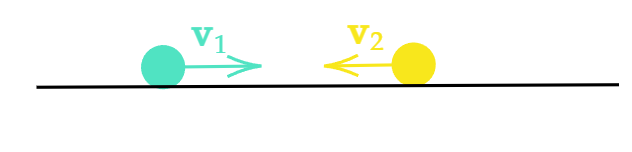
\includegraphics[width=0.4\textwidth]{Content/Figure/collision.png}
\end{figure}
\pause
\begin{columns}
\begin{column}{0.5\textwidth}
\scriptsize
Định luật bảo toàn động lượng:
\begin{equation*}
    m_1 v_1 - m_2 v_2 = m_1 v_1' - m_2 v_2'.
\end{equation*}
Định luật bảo toàn năng lượng:
\begin{equation*}
    \frac{m_1 v_1^2}{2} + \frac{m_2 v_2^2}{2} = \frac{m_1 {v_1'}^2}{2} + \frac{m_2 {v_2'}^2}{2}.
\end{equation*}
\normalsize
\end{column}
\begin{column}{0.5\textwidth}
Giải hệ phương trình trên ta được:
\begin{equation}
    \begin{aligned}
    v_1' = \frac{(m_1 - m_2)v_1 + 2m_2 v_2}{m_1 + m_2},\\
    v_2' = \frac{(m_2 - m_1)v_2 + 2m_1 v_1}{m_1 + m_2}.
    \end{aligned}
\end{equation}
\end{column}
\end{columns}
\end{frame}

\section{Bất biến trong một số bài toán khác}
\begin{frame}
    \frametitle{Đơn cực từ}
    Xét sự chuyển động của một điện tích điểm \(q_e\), khối lượng \(m\) trong từ trường của một đơn cực từ giả tưởng nằm yên tại gốc toạ độ:
    \[\mathbf{B}=k\frac{q_m}{r^2}\hat{r}.\]
    \begin{itemize}
        \item Phương trình động lực học: \(m\mathbf{a}=q_e(\mathbf{v}\times\mathbf{B})\).
        \item Công suất của lực từ bằng 0: \(\lvert\mathbf{v}\rvert=const\).
    \end{itemize}
    Chứng minh được rằng, đại lượng \[\mathbf{Q}=\mathbf{L}-kq_e q_m \hat{r}\] là một hằng số chuyển động (bất biến).
\end{frame}
\begin{frame}
    \frametitle{Đơn cực từ}
    \begin{columns}
        \begin{column}{0.5\textwidth}
            \vspace{-16pt}

            \begin{figure}
        \centering
        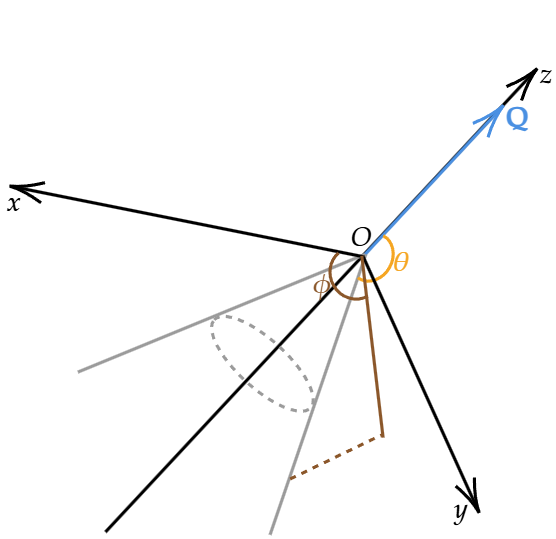
\includegraphics[width=6cm, height=6cm]{Content/Figure/magnetic_monopole.png}
    \end{figure}
        \end{column}
        \begin{column}{0.5\textwidth}
            \begin{itemize}
                \item \(\mathbf{Q}\cdot\hat{\phi}=mr^2\dot\theta=0\implies \theta=const\).
                \item \(\mathbf{Q}\cdot\hat{r}=Q\cos\theta=-kq_e q_m \implies \lvert \mathbf{Q}\rvert =const\).
                \item \(r(\phi)=\frac{Q\sin\theta}{mv\cos((\phi-\phi_0)\sin\theta)}\).
            \end{itemize}
            
        \end{column}
    \end{columns}
\end{frame}

\begin{frame}
\frametitle{Bất biến đoạn nhiệt}
Một vật nhỏ có khối lượng \(m\) chuyển động và va chạm đàn hồi với hai vạch tường cách nhau một khoảng \(L\). Dịch chuyển vách tường bên phải lại một cách rất chậm. Tìm liên hệ giữa vận tốc \(v\) của vật và độ dịch chuyển \(x\) của tường.
\begin{figure}
    \centering
    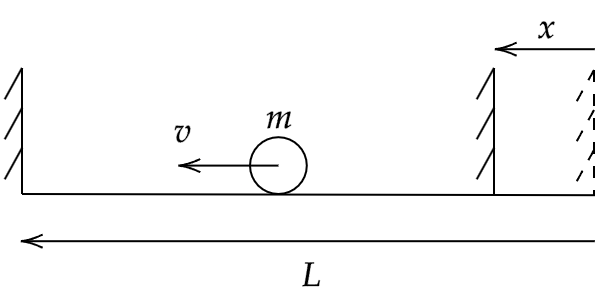
\includegraphics[width=0.5\textwidth]{Content/Figure/adiabatic.png}
\end{figure}
\end{frame}

\begin{frame}
\frametitle{Bất biến đoạn nhiệt}
Sau mỗi va chạm, tường truyền cho vật một động lượng \(\Delta p = 2mv\).

Tường giống như tác dụng một "lực" \(F\) lên vật:
\begin{equation*}
    F=\frac{\Delta p}{\Delta t}=\frac{2mv}{\frac{2(L-x)}{v}}.
\end{equation*}
Định lí công - động năng:
\begin{equation*}
    d\left(\frac{mv^2}{2}\right)=F dx=\frac{mv^2}{L-x}dx.
\end{equation*}
Chuyển vế và nguyên hàm, ta thu được:
\begin{equation}
    v(L-x)=const.
\end{equation}
\end{frame}
\begin{frame}
    \frametitle{Một ``nghịch lý''}
    Một quả tên lửa có thể cung cấp vận tốc \(u\), tức năng lượng bằng \(\frac{mu^2}{2}\) cho đầu đạn sau khi đốt hết nhiên liệu. Vậy nếu như tên lửa được phóng từ một máy bay đang bay
    với vận tốc \(v\), vận tốc của đầu đạn sẽ là \(v+u\). Như vậy động năng tổng cộng của đầu đạn lúc này là \[\frac{m(v+u)^2}{2}>\frac{mu^2}{2}+\frac{mv^2}{2}.\] Trong khi ta biết rằng tổng hoá năng của nhiên liệu là không đổi trong cả hai trường hợp, vậy lượng năng lượng này từ đâu r? 
    Coi rằng tổng khối lượng của nhiên liệu là rất nhỏ so với khối lượng của đầu đạn.
\end{frame}

\begin{frame}[allowframebreaks]{Tài liệu tham khảo}
    \begin{refsection}
        \nocite{morin2008introduction,calculusjame, 3b1b,griffiths2023introduction}
         \printbibliography
    \end{refsection}
\end{frame}


\end{document}